\documentclass[12pt]{standalone}
\usepackage[T1]{fontenc}
\usepackage{textcomp}
\usepackage{tikz}
\usetikzlibrary{calc}
\usepackage{tkz-euclide}
\usetkzobj{all} 

\title{MAT\\ CIRCLE\\ 2013.}

\begin{document}
  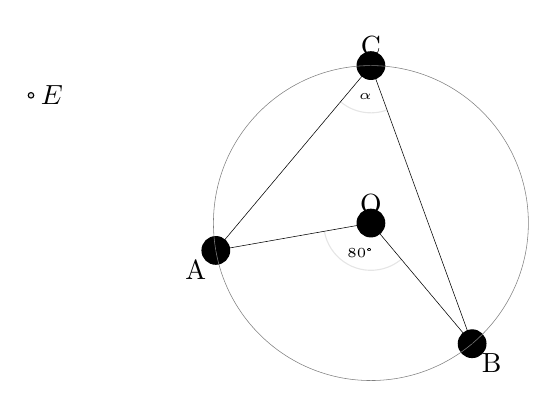
\begin{tikzpicture}
    \tkzDefPoint[label=above:O](0,0){O}
    \tkzDefPoint[label=below left:A](190:2){A}
    \tkzDefPoint[label=below right:B](310:2){B}
    \tkzDefPoint[label=above:C](90:2){C}
    \tkzDrawPoints[fill=black,size=10](O,A,B,C)
    \tkzDrawCircle(O,A)
    \tkzDrawPolygon(C,A,O,B)
    \tkzMarkAngle[fill=purple,opacity=0.1,size=0.6](A,O,B)
    \tkzLabelAngle[pos=0.4,font=\tiny](A,O,B){80\textdegree}
    \tkzMarkAngle[fill=purple,opacity=0.1,size=0.6](A,C,B)
    \tkzLabelAngle[pos=0.4,font=\tiny](A,C,B){$\alpha$}

    \coordinate (E) at ($(A)!1!90:(C)$);
    \tkzLabelPoints[right](E)
    \tkzDrawPoints(E)
  \end{tikzpicture}
  % \begin{tikzpicture}
  %   \tkzDefPoint[label=below right:S](0:0){O}
  %   \tkzDefPoint[label=above:A](80:2){A}
  %   \tkzDefPoint[label=left:B](190:2){B}
  %   \tkzDefPoint[label=right:C](3:2){C}
  %   \tkzDrawPoints[fill=black,size=10](O,A,B,C)
  %   \tkzDrawCircle(O,A)
  %   \tkzDrawPolygon(A,O,B,C)
  %   \tkzMarkAngle[fill=purple,opacity=0.1,size=0.6](A,O,B)
  %   \tkzLabelAngle[pos=-0.25,font=\tiny](A,O,B){$\beta$}
  %   \tkzMarkAngle[fill=purple,opacity=0.1,size=0.6](A,C,B)
  %   \tkzLabelAngle[pos=-0.35,font=\tiny](A,C,B){30\textdegree}
  % \end{tikzpicture}
  % \begin{tikzpicture}
  %   \tkzDefPoint(0:0){O}
  %   \tkzDefPoint[label=above:A](80:2){A}
  %   \tkzDefPoint[label=left:B](190:2){B}
  %   \tkzDefPoint[label=right:C](3:2){C}
  %   \tkzDefPoint[label=below:D](290:2){D}
  %   \tkzDrawPoints[fill=black,size=10](A,B,C,D)
  %   \tkzDrawCircle(O,A)
  %   \tkzDrawPolygon(A,D,B,C)
  %   \tkzMarkAngle[fill=purple,opacity=0.1,size=0.6](A,C,B)
  %   \tkzLabelAngle[pos=-0.4,font=\tiny](A,C,B){32\textdegree}
  %   \tkzMarkAngle[fill=purple,opacity=0.1,size=0.6](A,D,B)
  %   \tkzLabelAngle[pos=0.35,font=\tiny](A,D,B){$\beta$}
  % \end{tikzpicture}
\end{document}